% This is the Reed College LaTeX thesis template. Most of the work
% for the document class was done by Sam Noble (SN), as well as this
% template. Later comments etc. by Ben Salzberg (BTS). Additional
% restructuring and APA support by Jess Youngberg (JY).
% Your comments and suggestions are more than welcome; please email
% them to cus@reed.edu
%
% See http://web.reed.edu/cis/help/latex.html for help. There are a
% great bunch of help pages there, with notes on
% getting started, bibtex, etc. Go there and read it if you're not
% already familiar with LaTeX.
%
% Any line that starts with a percent symbol is a comment.
% They won't show up in the document, and are useful for notes
% to yourself and explaining commands.
% Commenting also removes a line from the document;
% very handy for troubleshooting problems. -BTS

% As far as I know, this follows the requirements laid out in
% the 2002-2003 Senior Handbook. Ask a librarian to check the
% document before binding. -SN

%%
%% Preamble
%%
% \documentclass{<something>} must begin each LaTeX document
\documentclass[12pt,twoside]{reedthesis}
% Packages are extensions to the basic LaTeX functions. Whatever you
% want to typeset, there is probably a package out there for it.
% Chemistry (chemtex), screenplays, you name it.
% Check out CTAN to see: http://www.ctan.org/
%%
\usepackage{graphicx,latexsym}
\usepackage{amsmath}
\usepackage{amssymb,amsthm}
\usepackage{longtable,booktabs,setspace}
\usepackage{chemarr} %% Useful for one reaction arrow, useless if you're not a chem major
\usepackage[hyphens]{url}
% Added by CII
\usepackage{hyperref}
\usepackage{lmodern}
% End of CII addition
\usepackage{rotating}

% Next line commented out by CII
%%% \usepackage{natbib}
% Comment out the natbib line above and uncomment the following two lines to use the new 
% biblatex-chicago style, for Chicago A. Also make some changes at the end where the 
% bibliography is included. 
%\usepackage{biblatex-chicago}
%\bibliography{thesis}


% Added by CII (Thanks, Hadley!)
% Use ref for internal links
\renewcommand{\hyperref}[2][???]{\autoref{#1}}
\def\chapterautorefname{Chapter}
\def\sectionautorefname{Section}
\def\subsectionautorefname{Subsection}
% End of CII addition

% Added by CII 
\usepackage{caption}
\captionsetup{width=5in}
% End of CII addition

% \usepackage{times} % other fonts are available like times, bookman, charter, palatino


% To pass between YAML and LaTeX the dollar signs are added by CII
\title{Statistical Inference on Random Forests}
\author{Aurora Owens}
% The month and year that you submit your FINAL draft TO THE LIBRARY (May or December)
\date{May 2017}
\division{Mathematics and Natural Sciences}
\advisor{Andrew Bray}
%If you have two advisors for some reason, you can use the following
% Uncommented out by CII
% End of CII addition

%%% Remember to use the correct department!
\department{Mathematics}
% if you're writing a thesis in an interdisciplinary major,
% uncomment the line below and change the text as appropriate.
% check the Senior Handbook if unsure.
%\thedivisionof{The Established Interdisciplinary Committee for}
% if you want the approval page to say "Approved for the Committee",
% uncomment the next line
%\approvedforthe{Committee}

% Added by CII
%%% Copied from knitr
%% maxwidth is the original width if it's less than linewidth
%% otherwise use linewidth (to make sure the graphics do not exceed the margin)
\makeatletter
\def\maxwidth{ %
  \ifdim\Gin@nat@width>\linewidth
    \linewidth
  \else
    \Gin@nat@width
  \fi
}
\makeatother

\renewcommand{\contentsname}{Table of Contents}
% End of CII addition

\setlength{\parskip}{0pt}

% Added by CII

\providecommand{\tightlist}{%
  \setlength{\itemsep}{0pt}\setlength{\parskip}{0pt}}

\Acknowledgements{
I want to thank a few people.
}

\Dedication{
You can have a dedication here if you wish.
}

\Preface{
This is an example of a thesis setup to use the reed thesis document
class.
}

\Abstract{
The preface pretty much says it all. \par  Second paragraph of abstract
starts here.
}

% End of CII addition
%%
%% End Preamble
%%
%

\begin{document}

% Everything below added by CII
      \maketitle
  
  \frontmatter % this stuff will be roman-numbered
  \pagestyle{empty} % this removes page numbers from the frontmatter

      \begin{acknowledgements}
      I want to thank a few people.
    \end{acknowledgements}
  
      \begin{preface}
      This is an example of a thesis setup to use the reed thesis document
      class.
    \end{preface}
  
      \hypersetup{linkcolor=black}
    \setcounter{tocdepth}{2}
    \tableofcontents
  
      \listoftables
  
      \listoffigures
  
      \begin{abstract}
      The preface pretty much says it all. \par  Second paragraph of abstract
      starts here.
    \end{abstract}
  
      \begin{dedication}
      You can have a dedication here if you wish.
    \end{dedication}
  
  \mainmatter % here the regular arabic numbering starts
  \pagestyle{fancyplain} % turns page numbering back on

  \chapter{Introduction}\label{introduction}
  
  \section{Trees and Random Forests}\label{trees-and-random-forests}
  
  \subsection{Trees}\label{trees}
  
  ~~~~~Decision trees may be familiar to many with a background in the
  social or medical sciences as convenient ways to represent data and can
  assist in decision making. Morgan and Sonquist (1963) derived a way for
  constructing trees motivated by the specific feature space of data
  collected from interviews and surveys. Unlike, say agricultural data
  which involves mostly numerical variables like rainfall, the data
  collected from interviews is mostly categorical. On top of this issue,
  the datasets Morgan and Sonquist dealt with had few participants,
  \emph{n}, and much data collected on them, \emph{p}. To continue with
  their list of difficulties, there was reason to believe that there were
  lurking errors in the variables that would be hard identify and
  quantify. Lastly, many of the predictors were correlated and Morgan and
  Sonquist doubted that the additive assumptions of many models would be
  appropriate for this data. Morgan and Sonquist noted that while many
  statistical methods would have difficulty accurately parsing this data,
  a clever researcher with quite a lot of time could create a suitable
  model simply by grouping values in the feature space and predicting that
  the response corresponding to these values would be the mean of the
  observed responses given the grouped conditions. Their formalization of
  this procedure in terms of ``decision rules'' laid the ground work for
  future research on decision trees.
  
  ~~~~~Later researchers proposed new methods for creating trees that
  improved upon the Morgan and Sonquist model. Leo Breiman et al 1984
  proposed an algorithm called CART, \emph{classification and regression
  trees}, that would allow trees to be fit on various types of data. An
  alternative to this method is conditional inference trees. Torsten
  Hothorn, Kurt Hornik, Achim Zeileis argue in their 2006 paper
  \emph{Unbiased Recursive Partitioning: A Conditional Inference
  Framework}, CART has a selection bias toward variables with either
  missing values or a great number of possible splits. This bias can
  effect the interpretability of all tree models fit using this method. As
  an alternative to CART and other algorithms, Hothorn et al propose a new
  method, conditional inference trees.
  
  ~~~~~ There is a limit to the predictive capabilities of a single tree
  as they suffer from high variance. To alleviate this, random forests are
  often used instead. They function by enlisting the help of many trees,
  and then by aggregating the responses over all of them but with a subtle
  trick that ensures the trees will be independent of each other. At each
  split only \emph{m} variables are considered as possible candidates.
  Random forests and their algorithms will be discussed at length in
  Chapter 2.
  
  \section{What We Mean When We Talk About
  Inference}\label{what-we-mean-when-we-talk-about-inference}
  
  \subsection{Inferential vs Descriptive
  Statistics}\label{inferential-vs-descriptive-statistics}
  
  ~~~~~ A note should be made of the difference between inferential and
  descriptive statistics. This paper's aim is to describe a process of
  making inferential claims using random forests, not descriptive ones.
  Descriptive statistics describe the data at hand without making any
  reference to a larger data generating system that they come from. It
  follows that inferential statistics then make claims about the data
  generating system given the data at hand.
  
  ---Frequentist vs Bayesian---
  
  ~~~~~ ---There is some debate about interpreting inferential statistics.
  On one hand, we have the Bayesian model---
  
  \emph{Need a better way to discuss inference than Bayes/frequentist}
  
  \section{Permutations and
  Populations}\label{permutations-and-populations}
  
  ~~~~~ As stated in the introduction of the \emph{Chronical of
  Permutations Statistical Methods} by KJ Berry et al, 2014, there are two
  models of statistical inference. One is the population model, where we
  assume that the data was randomly sampled from one (or more)
  populations. Under this model, we assume that the data generated follows
  some known distribution. ``Under the population model, the level of
  statistical significance that results from applying a statistical test
  to the results of an experiment or a survey corresponds to the frequency
  with which the null hypothesis would be rejected in repeated random
  samplings from the same specified population(s)'', (Berry et al, 2014).
  
  ~~~~~The permutation family of methods, on the other hand, only assumes
  that the observed result was caused by experimental variability. The
  test statistics is first calculated for the observed data, then the data
  is permuted a number of times. The statistic is calculated after each
  permutation to dervive a distribution of possible values. Then the
  original test statistic is tested against this distribution. If it is
  exceptionally rare, then there is evidence that our observation was not
  simply experimental variability.
  
  \section{Inference on Random Forests}\label{inference-on-random-forests}
  
  \subsection{The Problem}\label{the-problem}
  
  ~~~~~Random forests create models with great predictive-, but poor
  inferential capabilities. After Morgan and Sonquist initial development
  of decision trees, they quickly moved to the domain of machine learning
  and away from statistics, thus, researchers focused on bettering
  predictions and improving run times and less on the statistics behind
  them. Inferential statistics with random forests is usually treated as a
  variable selection problem, and generally falls behind the predictions
  in importance. This has limited the applications of random forests in
  certain fields, as to many the question of ``why'' the data is the way
  it is, is just, if not more, important as the predictions. There are
  several means of performing descriptive statistics with random forests
  that could be interpreted incorrectly as attempting to answer this,
  namely base variable importance, but without a statistically backed
  method for performing variable importance, the use of random forest is
  limited to prediction-only settings.
  
  \subsection{Proposed solutions to this
  problem}\label{proposed-solutions-to-this-problem}
  
  ~~~~~Statisticians Breiman and Cutler proposed a method of permuted
  variable importance to answer this problem. Their method compares the
  variable importance for each variable in a tree-wise manner. For each
  tree, the permuted variable importance of the variable \(X_j\) is:
  
  \[PV^t(x_j) = \frac{\sum_{i \in |B|} {y} - \hat{y}^t}{|B|} - \frac{\sum_{i \in |*B|} {y} - \hat{*y}^t}{|*B|} \]
  
  ~~~~~ Where \(B\) is the matrix representing the feature space, \(|B|\)
  is the number of observations, \(*B\) is the matrix of predictors but
  with \(X_j\) permuted, \(\hat{y}\) is the predicted outcome, and
  \(\hat{*y}^t\) is the predicted outcomes after variable \(X_j\) has been
  permuted. This value is averaged over all the trees. It's important to
  note that if the variable \(X_j\) is not split on in the tree \(t\), the
  tree-wise variable importance will be 0.
  
  ~~~~~ Creating a permutation-based method is certainly an attractive
  solution to our problem. One, it allows us to estimate the distribution
  of variable importance and generate a Z score under the null hypothesis
  that \(PV = 0\).
  
  \[PV(x_j) = \frac{\sum_1^ntree PV^t(x_j)}{\frac{\hat{\sigma}}{\sqrt{ntree}}}\]
  
  ~~~~~ Strobl et al from the University of Munich criticize this method
  in their 2008 technical report, \textbf{Danger: High Power! -- Exploring
  the Statistical Properties of a Test for Random Forest Variable
  Importance}. One, this method has the downside of increasing power with
  increasing numbers of trees in the forest. This is a more or less
  arbitrary parameter which we would hope would not affect our importance
  estimates. Secondly, the null hypothesis under Breiman and Cutler's
  strategy is that the variable importance \(V\) for any variable \(X_j\)
  is not equal to zero given \(Y\), the response. Because random forests
  are most often used in situations with multicolinearity that would make
  other methods like the linear model difficult, Strobl argues that any
  variable importance measure worth its salt should not be mislead by
  correlation within the predictors.
  
  ~~~~~ The researchers at the University of Munich published a fully
  fleshed response to the Breiman and Cutler method in 2008, titled
  \emph{Conditional Variable Importance for Random Forests} that address
  these issues. Strobl et al propose restructuring the Breiman and Cutler
  algorithm to account for conditional dependence among the predictors.
  Their algorithm looks like this:
  
  \begin{enumerate}
  \def\labelenumi{\arabic{enumi}.}
  \tightlist
  \item
    Fit a random forest to the model, \(R_0\), and calculate base variable
    importance for each variable \(V\)
  \item
    For every predictor \(X_j \in X_1,...,X_n\):
  \end{enumerate}
  
  \begin{itemize}
  \tightlist
  \item
    2a. Conditionally permute \(X_j\) given the splits found in \(R_0\)
  \item
    2b. Fit a new random forest \(R_j\) with the permuted data
  \item
    2c. Calculate a new variable importance \(\hat{V}_j\)
  \end{itemize}
  
  \begin{enumerate}
  \def\labelenumi{\arabic{enumi}.}
  \setcounter{enumi}{2}
  \tightlist
  \item
    For every variable \(X_1,..., X_n\), \[CV(X_j) = \hat{V}_j - V_j\]
  \end{enumerate}
  
  ~~~~~ The null hypothesis is that \(CV(X_j) = 0\) given the predictor
  \(Y\) \emph{and all other predictors} \(X_1,..X_n\).This accounts for
  interactions between \(X_j\) and the other predictors. Using the
  simulated data from the previous example, here's an implementation of
  the algorithm outlined here as it is in the \texttt{party} package.
  
  ~~~~~This paper aims to provide a response to this method. One the
  conditional permutation algorithm is notoriously slow with any dataset
  of a size that is appropriate for a random forest. Two, the partitions
  are made from the random forest corresponding to the formula of
  \(Y~X_1,...,X_n\) instead of a model of \(X_j~X_1,...,X_n\).
  
  \chapter{Simulations and Comparisons}\label{simulations-and-comparisons}
  
  \section{Simulated Data}\label{simulated-data}
  
  \begin{itemize}
  \tightlist
  \item
    From Strobl et al:
  \end{itemize}
  
  ~~~~~To aid in comparisons between the methods, one of the simulated
  datasets considered in this paper will be generated from the same method
  as used in (Strobl et al, 2008???). Under this method, the 13 x 1000
  data set, \(D_1\), has 12 predictors, \(V_1,..,V_{12}\), where
  \(V_j \sim N(0,1)\). The first four are, however, block correlated to
  each other with \(\rho = .9\). They are related to \(Y\) by the linear
  equation:
  \[Y = 5 \cdot V_1 + 5 \cdot V_2 + 2 \cdot V_3 + 0 \cdot V_4 + -5 \cdot V_5 + -5\cdot V_6 + 0\cdot V_7 + 0 \cdot ..... + E, E \sim N(0,\frac 1 2 )\]
  Note that the coefficents for \(V_7,...,V_{12}\) are all zero.
  
  \begin{center}\includegraphics{Thesis_files/figure-latex/stroblSimPlot-1} \end{center}
  
  Let's move on to a more difficult situation. The dataset \(D2\) contains
  five predictors, \(X_1,...X_5\), that have an interesting structure-
  several of the predictors are correlated, but are not one -to -one. This
  violates an important assumtion of the linear model and means that these
  variables have low correlation. Note that this only makes sense in
  higher dimensions where we are estimating the value of \(X_j\) given
  \(X_1,...,X_n\).
  
  \begin{Shaded}
  \begin{Highlighting}[]
  \NormalTok{x1 <-}\StringTok{ }\KeywordTok{rnorm}\NormalTok{(}\DecValTok{1000}\NormalTok{)}
  
  \NormalTok{x2 <-}\StringTok{ }\DecValTok{2}\NormalTok{*}\KeywordTok{sqrt}\NormalTok{(}\KeywordTok{abs}\NormalTok{(x1)) +}\StringTok{ }\KeywordTok{rnorm}\NormalTok{(}\DecValTok{1000}\NormalTok{)}
  
  \NormalTok{x3 <-}\StringTok{ }\NormalTok{x1 +}\StringTok{ }\DecValTok{2}\NormalTok{*x2 +}\StringTok{ }\KeywordTok{rnorm}\NormalTok{(}\DecValTok{1000}\NormalTok{)}
  
  \NormalTok{x4 <-}\StringTok{ }\KeywordTok{rnorm}\NormalTok{(}\DecValTok{1000}\NormalTok{)}
  
  \NormalTok{x5 <-}\StringTok{ }\DecValTok{2}\NormalTok{*}\KeywordTok{sqrt}\NormalTok{(}\KeywordTok{abs}\NormalTok{(x4)) +}\StringTok{ }\KeywordTok{rnorm}\NormalTok{(}\DecValTok{1000}\NormalTok{)}
  
  \NormalTok{y <-}\StringTok{ }\NormalTok{x1 +}\StringTok{ }\DecValTok{2}\NormalTok{*x2 +}\StringTok{ }\DecValTok{3} \NormalTok{*}\StringTok{ }\NormalTok{x3 +}\StringTok{ }\DecValTok{4}\NormalTok{*x4 +}\StringTok{ }\DecValTok{1}\NormalTok{*x5 +}\StringTok{ }\KeywordTok{rnorm}\NormalTok{(}\DecValTok{1000}\NormalTok{)}
  
  \NormalTok{d2 <-}\StringTok{ }\KeywordTok{data.frame}\NormalTok{(y,x1,x2,x3,x4,x5)}
  
  \KeywordTok{cor}\NormalTok{(d2)}
  \end{Highlighting}
  \end{Shaded}
  
  \begin{verbatim}
             y         x1          x2          x3          x4         x5
  y  1.0000000 0.37370066  0.81852208  0.92926643  0.30615522 0.15357237
  x1 0.3737007 1.00000000  0.01253512  0.37828457  0.02553116 0.01196494
  x2 0.8185221 0.01253512  1.00000000  0.85944303 -0.04770287 0.04253338
  x3 0.9292664 0.37828457  0.85944303  1.00000000 -0.03116991 0.04579883
  x4 0.3061552 0.02553116 -0.04770287 -0.03116991  1.00000000 0.01984835
  x5 0.1535724 0.01196494  0.04253338  0.04579883  0.01984835 1.00000000
  \end{verbatim}
  
  \begin{Shaded}
  \begin{Highlighting}[]
  \KeywordTok{plot}\NormalTok{(d2)}
  \end{Highlighting}
  \end{Shaded}
  
  \begin{center}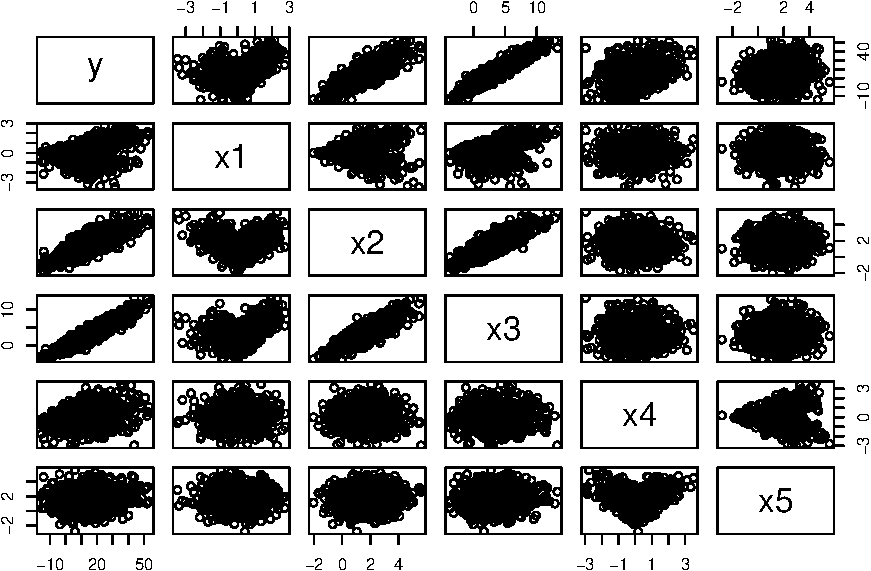
\includegraphics{Thesis_files/figure-latex/sqrtAbs-1} \end{center}
  
  The tricker relationship between the variables in \(D2\) was because
  they were generated using the square root of the absolute value of the
  other variable. Here, in \(D3\) the process is repeated but with the log
  of the absolute value.
  
  \begin{Shaded}
  \begin{Highlighting}[]
  \NormalTok{w1 <-}\StringTok{ }\KeywordTok{rnorm}\NormalTok{(}\DecValTok{1000}\NormalTok{)}
  
  \NormalTok{w2 <-}\StringTok{ }\DecValTok{2}\NormalTok{*}\KeywordTok{log}\NormalTok{(}\KeywordTok{abs}\NormalTok{(w1)) +}\StringTok{ }\KeywordTok{rnorm}\NormalTok{(}\DecValTok{1000}\NormalTok{)}
  
  \NormalTok{w3 <-}\StringTok{ }\NormalTok{w1 +}\StringTok{ }\DecValTok{2}\NormalTok{*w2 +}\StringTok{ }\KeywordTok{rnorm}\NormalTok{(}\DecValTok{1000}\NormalTok{)}
  
  \NormalTok{w4 <-}\StringTok{ }\KeywordTok{rnorm}\NormalTok{(}\DecValTok{1000}\NormalTok{)}
  
  \NormalTok{w5 <-}\StringTok{ }\DecValTok{2}\NormalTok{*}\KeywordTok{log}\NormalTok{(}\KeywordTok{abs}\NormalTok{(w4)) +}\StringTok{ }\KeywordTok{rnorm}\NormalTok{(}\DecValTok{1000}\NormalTok{)}
  
  \NormalTok{y <-}\StringTok{ }\NormalTok{w1 +}\StringTok{ }\DecValTok{2}\NormalTok{*w2 +}\StringTok{ }\DecValTok{3} \NormalTok{*}\StringTok{ }\NormalTok{w3 +}\StringTok{ }\DecValTok{4}\NormalTok{*w4 +}\StringTok{ }\DecValTok{1}\NormalTok{*w5 +}\StringTok{ }\KeywordTok{rnorm}\NormalTok{(}\DecValTok{1000}\NormalTok{)}
  
  \NormalTok{d3 <-}\StringTok{ }\KeywordTok{data.frame}\NormalTok{(y,w1,w2,w3,w4,w5)}
  
  \KeywordTok{cor}\NormalTok{(d3)}
  \end{Highlighting}
  \end{Shaded}
  
  \begin{verbatim}
              y          w1          w2          w3          w4          w5
  y  1.00000000  0.15728407  0.94764704  0.97416878  0.17279746  0.05578763
  w1 0.15728407  1.00000000 -0.02714818  0.15752508  0.03050113 -0.05109218
  w2 0.94764704 -0.02714818  1.00000000  0.96531545 -0.01975103 -0.04414540
  w3 0.97416878  0.15752508  0.96531545  1.00000000 -0.01042494 -0.05419898
  w4 0.17279746  0.03050113 -0.01975103 -0.01042494  1.00000000 -0.03325170
  w5 0.05578763 -0.05109218 -0.04414540 -0.05419898 -0.03325170  1.00000000
  \end{verbatim}
  
  \begin{Shaded}
  \begin{Highlighting}[]
  \KeywordTok{plot}\NormalTok{(d3)}
  \end{Highlighting}
  \end{Shaded}
  
  \begin{center}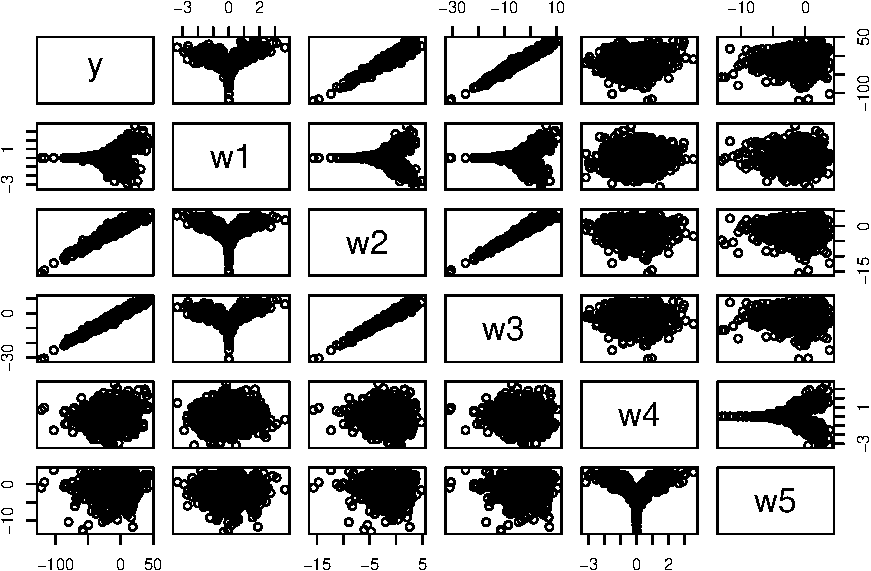
\includegraphics{Thesis_files/figure-latex/logAbs-1} \end{center}
  
  \section{Models and Comparisons}\label{models-and-comparisons}
  
  \section{Trees}\label{trees-1}
  
  \subsection{CART}\label{cart}
  
  In 1984, Breiman et al introduces a revolutionary new algorithm for
  trees. \textbf{Need to acquire} \emph{Classification and Regression
  Trees} \textbf{to make sure the method discused in MASS is the same that
  Breiman uses/is used in} \texttt{randomForest}
  
  \textbf{Tree Algorithm} CART?
  
  Begin by considering the entire feature space \(X_1, ..., X_n\). Then:
  
  \begin{enumerate}
  \def\labelenumi{\arabic{enumi}.}
  \item
    Consider every possible pair of partitions of this feature space,
    \(P_1, P_2\), so that if \(X_1 = x_1 , X_2 = x_2,..., X_n = x_n\)
    where \({x_1,...,x_n} \in P_1\) then our prediction is the mean value
    of \(y\) given \(x_1,..,x_n \in P_1\).
  \item
    Choose the partitions that minimize RSS
  \item
    For each new partition, repeat steps 1 and 2 until some stopping
    condition is reached.
  \end{enumerate}
  
  \subsection{Binary Recursive
  Partitioning}\label{binary-recursive-partitioning}
  
  \subsection{Conditional Inference
  Trees}\label{conditional-inference-trees}
  
  CI trees 1. For case weights \(w\) test the global null hypothesis of
  independence between any of the m covariates and the response. Stop if
  this hypothesis cannot be rejected. Otherwise select the \(j_{th}\)
  covariate \(Xj\) with strongest association to \(Y\).
  
  \begin{enumerate}
  \def\labelenumi{\arabic{enumi}.}
  \setcounter{enumi}{1}
  \item
    Choose a set \(A \subset X_{j}\) in order to split \(X_{j}\) into two
    disjoint sets \(A\) and \(X_{j}\) ~\(A\). The case weights
    \(w_{left}\) and \(w_{right}\) determine the two subgroups with
    \(w_{left,i} = w_iI(X_{j\cdot i} \in A)\) and
    \(w_{right,i} = w_iI(X_{ji} \in A)\) for all \(i = 1,...,n\) (
    \(I(·)\) denotes the indicator function).
  \item
    Recursively repeat steps 1 and 2 with modified case weights \(w_left\)
    and \(w_right\), respectively.
  \end{enumerate}
  
  from
  \url{https://eeecon.uibk.ac.at/~zeileis/papers/Hothorn+Hornik+Zeileis-2006.pdf}
  
  After step 1 is completed, any goodness of fit method can be used to
  generate the split and choose the set \(A\). Note that in this method
  the splitting is done separately from the variable selection.
  
  \section{Bagged Forests}\label{bagged-forests}
  
  \section{Random Forests}\label{random-forests}
  
  \chapter{Permuatations Tests Theory and Application to Conditional
  Variable
  Importance}\label{permuatations-tests-theory-and-application-to-conditional-variable-importance}
  
  \chapter{Implementation of Our
  Method}\label{implementation-of-our-method}
  
  \chapter*{Conclusion}\label{conclusion}
  \addcontentsline{toc}{chapter}{Conclusion}
  
  \setcounter{chapter}{4} \setcounter{section}{0}
  
  If we don't want Conclusion to have a chapter number next to it, we can
  add the \texttt{\{.unnumbered\}} attribute. This has an unintended
  consequence of the sections being labeled as 3.6 for example though
  instead of 4.1. The \LaTeX~commands immediately following the Conclusion
  declaration get things back on track.
  
  \subsubsection{More info}\label{more-info}
  
  And here's some other random info: the first paragraph after a chapter
  title or section head \emph{shouldn't be} indented, because indents are
  to tell the reader that you're starting a new paragraph. Since that's
  obvious after a chapter or section title, proper typesetting doesn't add
  an indent there.
  
  \appendix
  
  \chapter{The First Appendix}\label{the-first-appendix}
  
  This first appendix includes all of the R chunks of code that were
  hidden throughout the document (using the \texttt{include\ =\ FALSE}
  chunk tag) to help with readibility and/or setup.
  
  \subsubsection{In the main Rmd file:}\label{in-the-main-rmd-file}
  
  \begin{Shaded}
  \begin{Highlighting}[]
  \CommentTok{# This chunk ensures that the reedtemplates package is}
  \CommentTok{# installed and loaded. This reedtemplates package includes}
  \CommentTok{# the template files for the thesis and also two functions}
  \CommentTok{# used for labeling and referencing}
  \NormalTok{if(!}\KeywordTok{require}\NormalTok{(devtools))}
    \KeywordTok{install.packages}\NormalTok{(}\StringTok{"devtools"}\NormalTok{, }\DataTypeTok{repos =} \StringTok{"http://cran.rstudio.com"}\NormalTok{)}
  \NormalTok{if(!}\KeywordTok{require}\NormalTok{(reedtemplates))\{}
    \KeywordTok{library}\NormalTok{(devtools)}
    \NormalTok{devtools::}\KeywordTok{install_github}\NormalTok{(}\StringTok{"ismayc/reedtemplates"}\NormalTok{)}
  \NormalTok{\}}
  \KeywordTok{library}\NormalTok{(reedtemplates)}
  \end{Highlighting}
  \end{Shaded}
  
  \subsubsection{\texorpdfstring{In
  \protect\hyperlink{ref_labels}{}:}{In :}}\label{in}
  
  \begin{Shaded}
  \begin{Highlighting}[]
  \CommentTok{# This chunk ensures that the reedtemplates package is}
  \CommentTok{# installed and loaded. This reedtemplates package includes}
  \CommentTok{# the template files for the thesis and also two functions}
  \CommentTok{# used for labeling and referencing}
  \NormalTok{if(!}\KeywordTok{require}\NormalTok{(devtools))}
    \KeywordTok{install.packages}\NormalTok{(}\StringTok{"devtools"}\NormalTok{, }\DataTypeTok{repos =} \StringTok{"http://cran.rstudio.com"}\NormalTok{)}
  \NormalTok{if(!}\KeywordTok{require}\NormalTok{(dplyr))}
      \KeywordTok{install.packages}\NormalTok{(}\StringTok{"dplyr"}\NormalTok{, }\DataTypeTok{repos =} \StringTok{"http://cran.rstudio.com"}\NormalTok{)}
  \NormalTok{if(!}\KeywordTok{require}\NormalTok{(ggplot2))}
      \KeywordTok{install.packages}\NormalTok{(}\StringTok{"ggplot2"}\NormalTok{, }\DataTypeTok{repos =} \StringTok{"http://cran.rstudio.com"}\NormalTok{)}
  \NormalTok{if(!}\KeywordTok{require}\NormalTok{(reedtemplates))\{}
    \KeywordTok{library}\NormalTok{(devtools)}
    \NormalTok{devtools::}\KeywordTok{install_github}\NormalTok{(}\StringTok{"ismayc/reedtemplates"}\NormalTok{)}
    \NormalTok{\}}
  \KeywordTok{library}\NormalTok{(reedtemplates)}
  \CommentTok{#flights <- read.csv("data/flights.csv")}
  \end{Highlighting}
  \end{Shaded}
  
  \chapter{The Second Appendix, for
  Fun}\label{the-second-appendix-for-fun}
  
  \backmatter
  
  \chapter{References}\label{references}
  
  \noindent
  
  \setlength{\parindent}{-0.20in} \setlength{\leftskip}{0.20in}
  \setlength{\parskip}{8pt}
  
  \hypertarget{refs}{}
  \hypertarget{ref-angel2000}{}
  Angel, E. (2000). \emph{Interactive computer graphics : A top-down
  approach with opengl}. Boston, MA: Addison Wesley Longman.
  
  \hypertarget{ref-angel2001}{}
  Angel, E. (2001a). \emph{Batch-file computer graphics : A bottom-up
  approach with quicktime}. Boston, MA: Wesley Addison Longman.
  
  \hypertarget{ref-angel2002a}{}
  Angel, E. (2001b). \emph{Test second book by angel}. Boston, MA: Wesley
  Addison Longman.


  % Index?

\end{document}

